\section{Energiflöde genom grunden}

% \subsubsection{Flöde vid termisk jämvikt}

Vid beräkningen av värmeflödet genom grunden användes geometrin som kan ses i figur \ref{fig:groundheat}.
Källaren antas vara belägen en halv meter under marknivån.

Som kan ses så varierar ej energiflödet så mycket mellan årstiderna och antags därför vara konstant i många applikationer.


\emph{\color{red} Nedanstående text måste göras om med de nya figurerna i åtanke,}
I samma figur ses även temperaturfördelningen vid termisk jämvikt då markens temperatur långt under huset sätts till konstanta $\unit[8]{^{circ}C}$. Vid markytan sattes konvektionskoefficienten till $h=\unit[15,5]{Wm^{-2}K^{-1}}$, motsvarande en ungefärlig vindhastighet (parallel med ytan) på $\unit[2]{ms^{-1}}$ vid utomhustemperaturen $\unit[0]{^{\circ}C}$. Källarens temperatur antas vara konstant $\unit[10]{^{\circ}C}$ och \textcolor{red}{grundens U-värde approximeras till $\unit[?]{Wm^{-2}K^{-1}}$}.


\begin{figure}
\centering
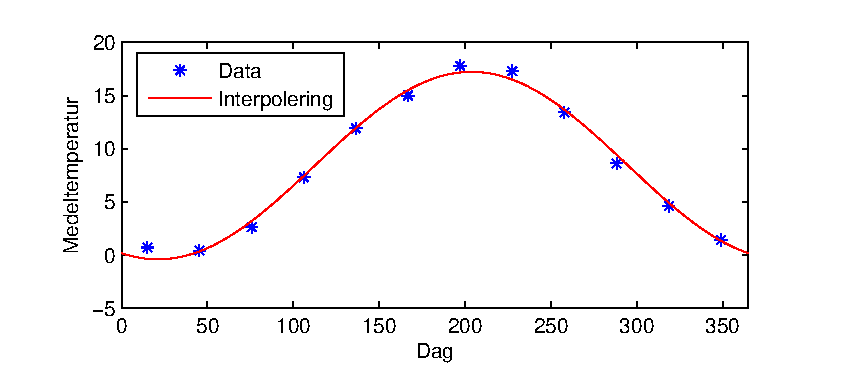
\includegraphics{images/meantemperature.eps}
\caption{Medeltemperaturen för göteborg de senaste 20 åren. Punkterna är data tagna från Miljöförvaltningen
och linjen är minstakvadratanpassningen som senare använts för att beräkna energiflöden.
\emph{\color{red} Denna graf kanske inte ska ligga här eller alls vara med. Metod möjligtvis? Vad tycker ni?}}
\end{figure}

\begin{figure}
\centering
\subfloat[Temperaturfördelningen i $^\circ\mbox{C}$ första januari.]{
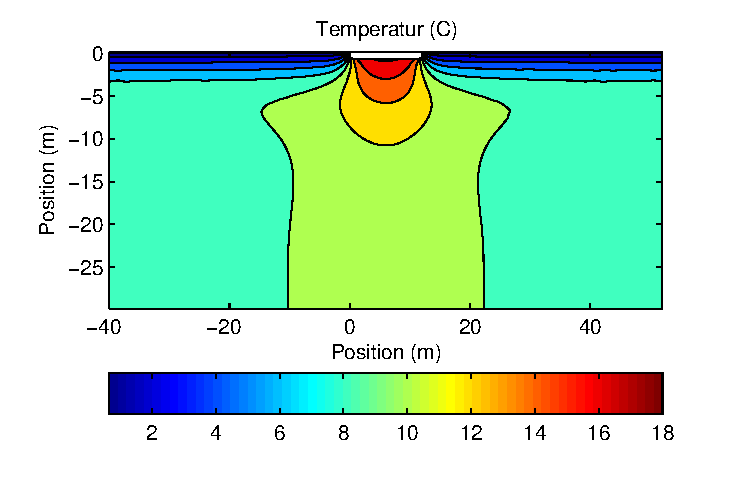
\includegraphics{images/groundheatdec.eps}
}

\subfloat[Temperaturfördelningen i $^\circ\mbox{C}$ första juli.]{
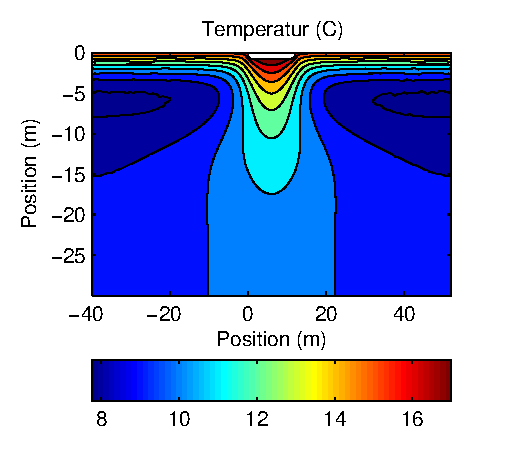
\includegraphics{images/groundheatjune.eps}
}
\caption{\label{fig:groundheat}Temperaturen i marken under en byggnad angivet i grader Celsius.
Temperaturfördelningarna skall motsvara två fiktiva dagar under ett år som är baserad på månadsmedeltemperaturen
de senaste 20 åren i Göteborg. Konvektionsparametern är satt till $h=15,5$. }
\end{figure}


\begin{figure}
\centering
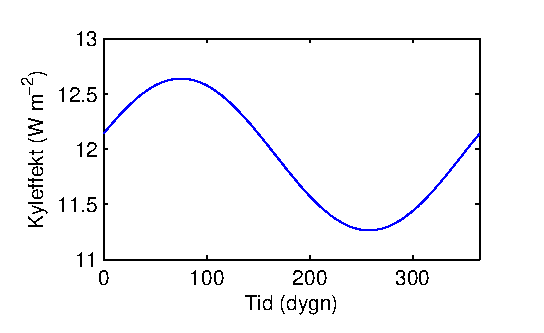
\includegraphics{images/groundcool.eps}
\caption{Kyleffekten per $m^2$ från grunden för medelåret de senaste tjugo åren. \emph{\color{red} Samma parametrar som figuren ovan.}\emph{\color{red}                                     
Detta är en viktig figur. Här kan ses att $\Delta Q = 1.5*22*13 = \unit[439]{W}$. Detta offsettas lätt genom att fler
människor befinner sig i fastigheten på vintern ty det är kallt ute eller fler kollar på tv istället för att sola.
Således finns det inget behov för att reglera framlednigstemperaturen för energiförluster från grunden. Kan antagas konstant
$\approx \unit[3,5]{kW}$. Låter denna siffra rimlig?}}

\end{figure}


% \subsubsection{Flöde vid transient förlopp}

Vid beräkningen av energiflödet genom grunden användes geometrin som kan ses i figur~\ref{fig:groundheat}. Grunden antas vara belägen en halv meter under marknivån. I resonomanget nedan kommer det att visa sig att marken reagerar så pass långsamt på temperaturförändringar att jämviktsläget är det enda relevanta. Ett transient förlopp är helt enkelt långt ifrån verkligheten. I beräkningarna här är konvektionsparametern satt till $h=15,5$.

Som kan ses i figur~\ref{fig:cooling_ground} så varierar inte energiflödet mer än en dryg watt per kvadratmeter mellan årstiderna och i många applikationer antas det därför vara konstant. Då vår grund är ungefär $\unit[22]{m}\cdot\unit[13]{m}=\unit[286]{m^2}$ ger detta ett energiutflöde mellan $\unit[3,6]{kW}$ på våren och $\unit[3,2]{kW}$ under tidig höst. 

\begin{figure}
\centering
\subfloat[Temperaturen i marken den första januari, $^\circ\mbox{C}$.]{
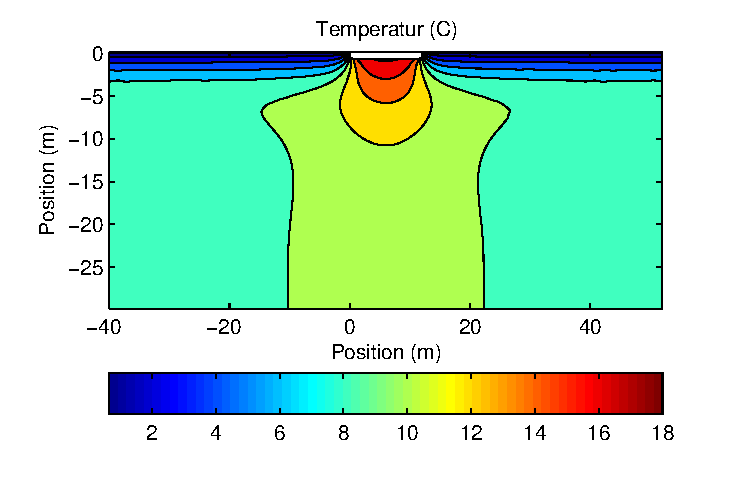
\includegraphics[width=7cm]{images/groundheatdec.eps}
}
\subfloat[Temperaturen i marken den första juli, $^\circ\mbox{C}$.]{
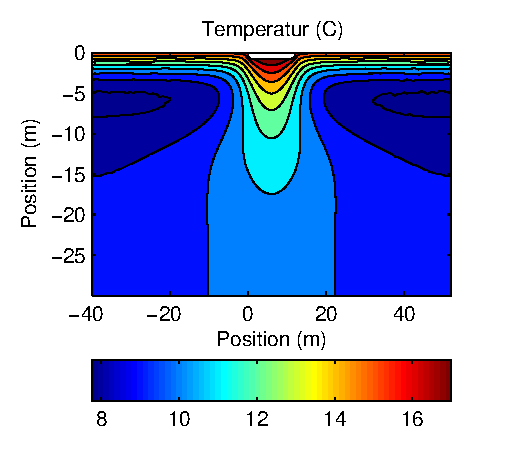
\includegraphics[width=7cm]{images/groundheatjune.eps}
}
\caption{\label{fig:groundheat}
Temperaturen i marken under byggnaden, $\unit{^\circ C}$, beräknat utifrån månadsmedeltemperaturen de senaste 20 åren i Göteborg för två fiktiva dagar i juni respektive januari. }
\end{figure}


\begin{figure}
\centering
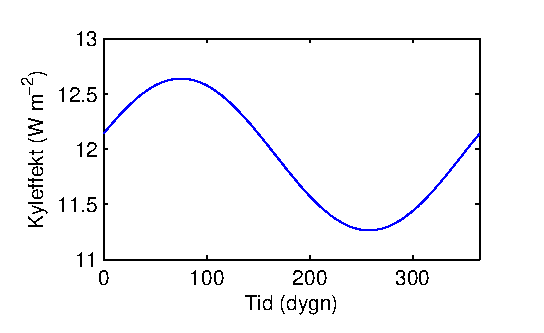
\includegraphics{images/groundcool.eps}
\caption{\label{fig:cooling_ground}
Kyleffekten per kvadratmeter från grunden för medelåret de senaste tjugo åren. Konvektionsparametern är satt till $h=15,5$. }

\end{figure}

